\documentclass{school-22.211-notes}
\date{February 15, 2012}

\begin{document}
\maketitle

\lecture{Slowing Down with Resonance Absorption}
At the end of last lecture, we get a smooth flux vs. lethargy curve, with two peaks (the one in the higher energy is stronger), and a smooth curve inbetween. Now we are going to look at the middle resonance region. 

\topic{Setting Up A Resonance Model}
\subtopic{Model Assumptions}
For our resonance model, we use the Single Level Breit-Wigner(SLBW) and assume:
\begin{itemize}
  \item the only resonance isotope is U238;
  \item all resonances are well isolated;
  \item only s-wave interaction (scattering \& absorption);
  \item Reich-Moore parameters can be used in SLBW;
  \item treat as resolved only the lowest 14 s-wave resonances;
  \item generate simple `statistical model' for energies up to 10 keV, assuming an uniform spacing 25 eV\footnote{notice on a typical plot which is log-log, the spacing appears to be closer and closer as energy increases; though it is actually reasonable to assume that the spacing is uniform};
\end{itemize}

\subtopic{Resonance Data}
One place to get resonance data is from LANL's website. For instance, \href{http://t2.lanl.gov/cgi-bin/endf?2,151,/inet/WWW/data/data/ENDFB-VII-neutron/U/238}{U238 Resonance Parameters}. Among the tables, GN means $\Gamma_N$ with unit eV, and GG means $\Gamma_G$ in eV. Extract the energy range from 0 to 10 keV (ignore the negative resonance energies). 

\topic{SLBW: Capture and Scattering Resonances}
\subtopic{Resolved Region}
\begin{align}
\sigma_{\gamma} (E,T) &= \sqrt{\frac{E_0}{E}} \frac{2}{\Gamma} A \psi(x,\xi) \\
\sigma_{n} (E,T) &= \frac{2}{\Gamma} \left[ A \psi(x,\xi) + B \chi(x,\xi) \right] + \sigma_{\mathrm{potential}} 
\end{align}
To convert them into a form suitable for numerical calculation,
\begin{align}
\sigma_{\gamma} (E,T) &= \sqrt{\frac{E_0}{E}} \frac{\Gamma_n}{\Gamma} \frac{\Gamma_{\gamma}}{\Gamma} r \psi(x,\xi) \\
\sigma_{n} (E,T) &= \frac{\Gamma_n}{\Gamma} \frac{\Gamma_n}{\Gamma} \left[ r \psi(x,\xi) + q \chi(x,\xi) \right] + \sigma_{\mathrm{potential}} 
\end{align}
where
\begin{align}
\xi &= \Gamma \sqrt{\frac{A}{4 k T E_0}} \\
x &= \frac{2 (E-E_0)}{\Gamma} \\
r &= \frac{h^2}{2 \pi E_0} \frac{A+1}{A} &= \frac{2603911}{E_0} \frac{A+1}{A} \\
q &= \sqrt{ r \sigma_{\mathrm{potential}} } \\
\Gamma &= \Gamma_n + \Gamma_{\gamma} \\
\sigma_{\mathrm{potential}} &=  4 \pi R^2 
\end{align}
Notice there are many numerical representations of the $\psi, \chi$ functions. For now, we can use ....


\subtopic{Results}
It is important to notice that \textit{all resonances contribute to all energies, even though their contributions can be infinitesimally}. 

\subtopic{Unresolved Region}
We assume 25 eV resonance spacing, and assume
\begin{align}
\Gamma_{\gamma} &= 0.023 \eV \\
\Gamma_{n} = 0.05 \sqrt{\frac{E}{E_{\mathrm{last}}}}  \eV
\end{align}
in which $E_{\mathrm{last}}$ means the last energy used in the 14 resonance region. 

Notice that for the purpose of this excercise we assume this region to be unresolved, whereas in reality they are resolved. 





%%%%%%%%%%%%%%%%%%%%%%%%% Qualify Exam Start %%%%%%%%%%%%%%%%%%%%%%%%%%%%
\lecture{Facts For Qualify Exam}
\begin{enumerate}
\item Flux = $\frac{n}{\cm^2 \s}.$

\item Fast flux in hydrogen is around $10^{14}$ n/cm$^2$s, and on the order of $10^{12}$n/cm$^2$s for thermal flux. 

\item Capture cross-section as in Figure~\ref{capture-xs}: 
\begin{figure}
  \centering
  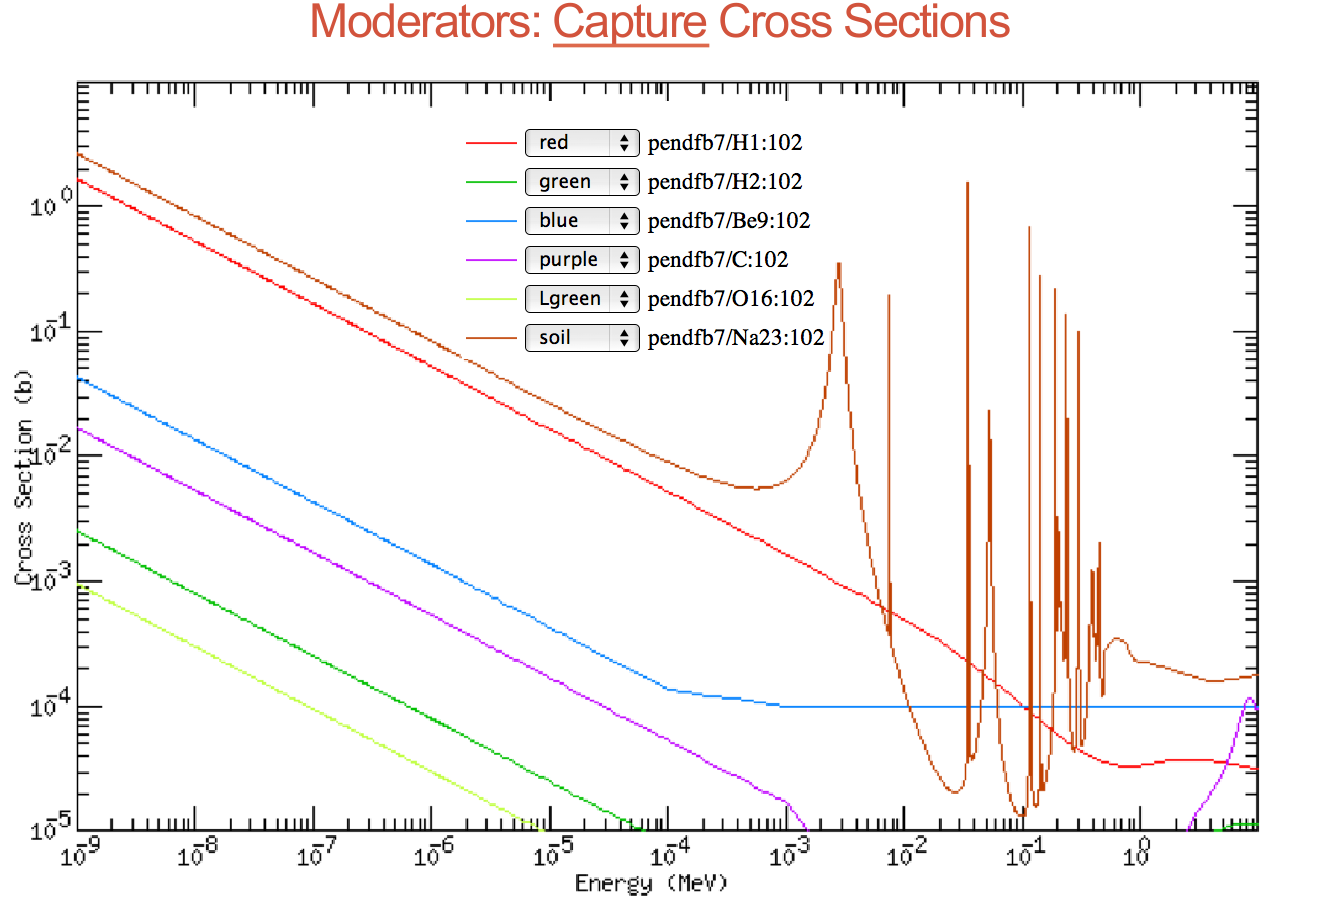
\includegraphics[width=4in]{images/capture-xs.png}
  \\
  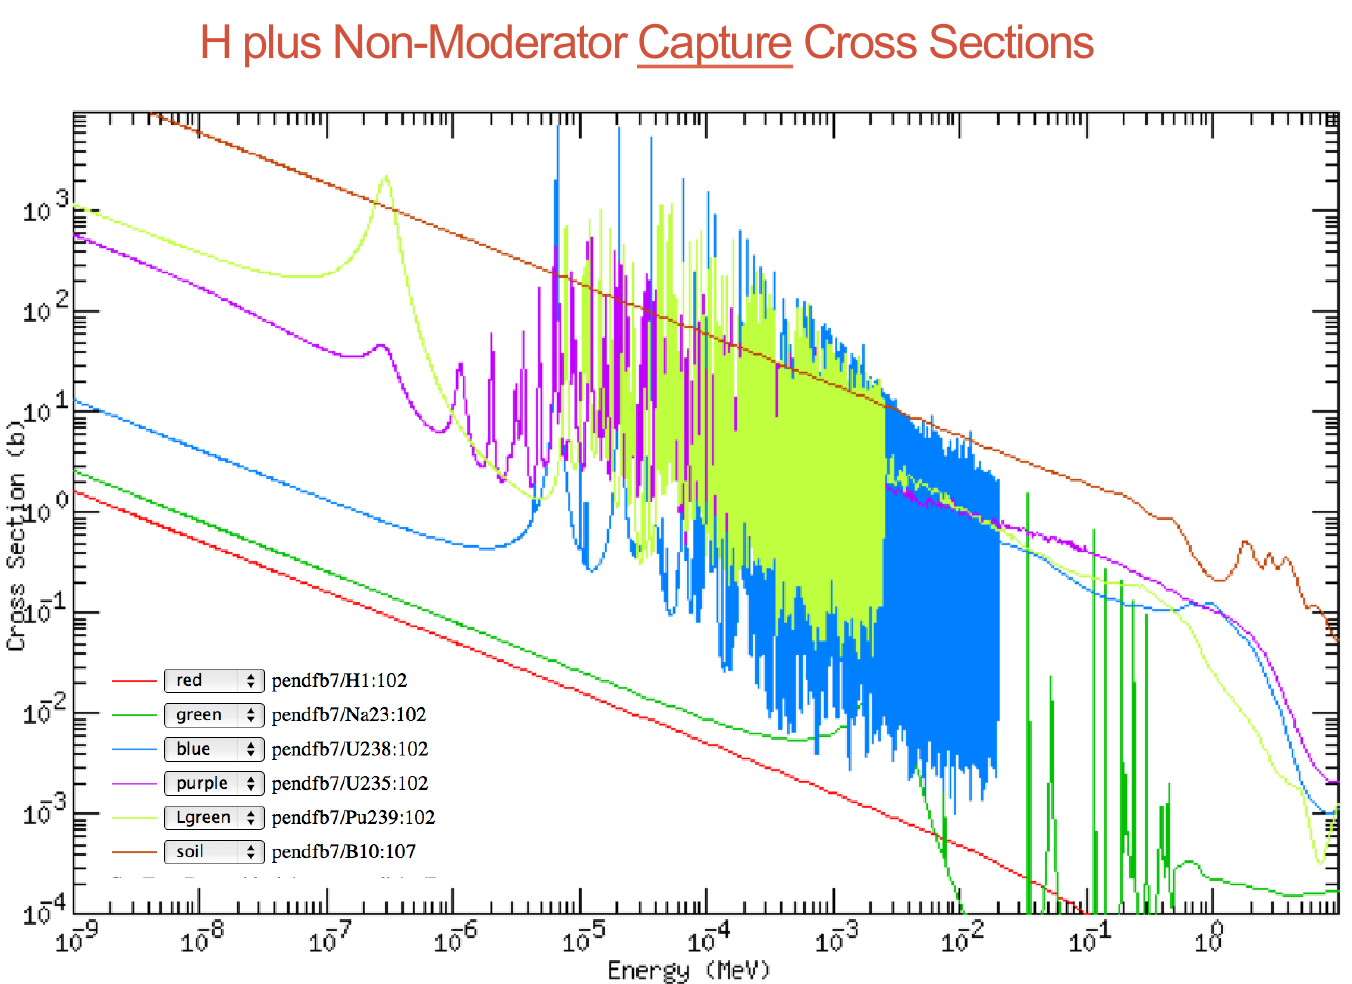
\includegraphics[width=4in]{images/capture-xs-2.png}
  \caption{Capture Cross Section} \label{capture-xs}
\end{figure}
\begin{enumerate}
\item H has no resonance; it has the highest scattering xs in LWR, so we can ignore any other isotopic's neutron scattering.   
\item Na has a huge resonance in 23 keV, and more resonances at higher energies because it is a heavy isotope.
\item Near zero energy,
\eqn{ \sigma(E\to 0) = }
\item Resonance at 6 to 7 eV: U238. 
\item U235's thermal elastic xs is larger than 238's, and they both have resonance around the same range.   
\item A small resonance at .3 eV: Pu239 (its signiture is a super low energy scattering xs). 
\end{enumerate}

\item Given an unknown material type, all we care is to count the nucleus density of each material and look at it's xs. 
\item Average fission neutron energy: 2 MeV; average peak fission energy: 1 MeV; see fission sepctrum. 
\end{enumerate}
%%%%%%%%%%%%%%%%%%%%%%%%% Qualify Exam End %%%%%%%%%%%%%%%%%%%%%%%%%%%%


\end{document}
